
%%%
% Things that happened after the experiments
%%%

\subsection{Round 1}

%%%
% Discussion of Round 1:
%	1. graphs to show how strategies were learned
%		4-5 frames to get a flip-book/transition to see things go on 1 strategy
%		2-3 different final strategy pngs
%	2. Performance:
%		worse than random agent in tournament play
%%%

%%%
Round 1 consisted of 32 agents with randomly allocated starting weights
paired off against each other.
%
These two agents played one million games against each other,
each starting with a random score,
learning and reinforcing their weight vectors after each game.
%%%

\subsubsection{Learning Process}

%%%
% Discuss flipbook figure
%%%

%%%
The results of the first round's training on a sample agent can be seen
in Figure~\ref{fig:r1_flip}.
%
Each individual square within the image represents the strength of a single
strategy,
in this case \handmaxavg,
where white means completely absent and black means completely dominant.
%
Each image was taken at an intermediate stage to capture and show transitions.
%%%

%%%
There are two things to note from these results.
%
The first is the stark contrast in colors in the majority of the image.
%
The other is the area in which these stark contrasts are present.
%%%

%%%
In the starting phase,
all weights are randomly assigned and relatively uniform with only slight
variances,
hence the blurry dull gray appearance.
%
As time progresses,
the image becomes crisper and filled with more contrast.
%
This indicates not only stronger preference for the strategy at the given
point,
but an almost all-or-nothing attitude towards adhering to a single strategy.
%
This means there is little to no nuance to which cards are chosen
and there is little to no chance for other strategies to collectively overrule 
or veto the major strategy.
%%%

%%%
Also of note is where the previously mentioned stark contrast is present and
where it is absent.
%
Since only those states which have been visited can have their weights
influenced,
the remainder will continue to stay untouched.
%
As can be seen in the top-right and bottom-left corners,
representing extremely unlikely scores to reach in which one player has
achieved a rather large lead while only allowing a few points,
contain only the dull gray of the initial weights.
%
This is because even with a potential spread of 60 points when initialized,
these outlandish scores are outside the realm of potential visitation.
%
Therefore, they have not been a part of any game,
so they cannot have their weights adjusted.
%%%

% Figure for the flipbook of strategies over time

\begin{figure}
\center

	\begin{subfigure}[t]{0.3\textwidth}
	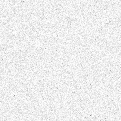
\includegraphics[width=\textwidth]{images/findings/round1/flipbook_a.png}
	\caption{Starting Weights}
	\end{subfigure}
	~
	\begin{subfigure}[t]{0.3\textwidth}
	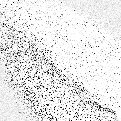
\includegraphics[width=\textwidth]{images/findings/round1/flipbook_b.png}
	\caption{After 200,000 games played}
	\end{subfigure}
	~
	\begin{subfigure}[t]{0.3\textwidth}
	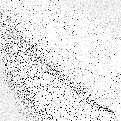
\includegraphics[width=\textwidth]{images/findings/round1/flipbook_c.png}
	\caption{After 400,000 games played}
	\end{subfigure}

	\begin{subfigure}[t]{0.3\textwidth}
	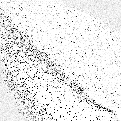
\includegraphics[width=\textwidth]{images/findings/round1/flipbook_d.png}
	\caption{After 600,000 games played}
	\end{subfigure}
	~
	\begin{subfigure}[t]{0.3\textwidth}
	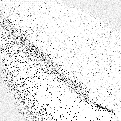
\includegraphics[width=\textwidth]{images/findings/round1/flipbook_e.png}
	\caption{After 800,000 games played}
	\end{subfigure}
	~
	\begin{subfigure}[t]{0.3\textwidth}
	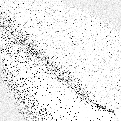
\includegraphics[width=\textwidth]{images/findings/round1/flipbook_f.png}
	\caption{Final Weights}
	\end{subfigure}

\caption{%
	Training weights representation for Agent 0's \handmaxavg\
	strategy when the agent is the dealer
	over the course of the one million games of Round 1.
	In these images, the y-axis represents the player's own score,
	the x-axis the opponent's score,
	with the origin starting at the top-left of the image.
	% N.B. This is correct of generated images from the python code
	%	as of 2018-03-08 19:12.
	% no later modifications will be made from the python code directly to
	% save myself the headache. maybe this will be converted later to be
	% more easily human understood
	% Rotate 90 deg counter-clockwise will make x=my_score, y=opp_score
}
% TODO: figure out axes
% TODO: change these images to hand_max_min: much starker contrast
\label{fig_r1-flip}
\end{figure}


\begin{figure}
\center

	\begin{subfigure}[t]{0.22\textwidth}
		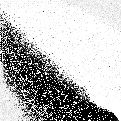
\includegraphics[width=\textwidth]{images/findings/round1/strategies_handmaxmin.png}
		\caption{\handmaxmin}
	\end{subfigure}
	~
	\begin{subfigure}[t]{0.22\textwidth}
		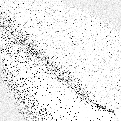
\includegraphics[width=\textwidth]{images/findings/round1/strategies_handmaxavg.png}
		\caption{\handmaxavg}
	\end{subfigure}
	~
	\begin{subfigure}[t]{0.22\textwidth}
		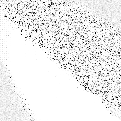
\includegraphics[width=\textwidth]{images/findings/round1/strategies_handmaxmed.png}
		\caption{\handmaxmed}
	\end{subfigure}
	~
	\begin{subfigure}[t]{0.22\textwidth}
		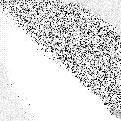
\includegraphics[width=\textwidth]{images/findings/round1/strategies_handmaxposs.png}
		\caption{\handmaxposs}
	\end{subfigure}

	\begin{subfigure}[t]{0.22\textwidth}
		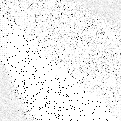
\includegraphics[width=\textwidth]{images/findings/round1/strategies_cribminavg.png}
		\caption{\cribminavg}
	\end{subfigure}
	~
	\begin{subfigure}[t]{0.22\textwidth}
		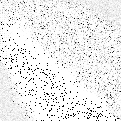
\includegraphics[width=\textwidth]{images/findings/round1/strategies_peggingmaxavggained.png}
		\caption{\peggingmaxavggained}
	\end{subfigure}
	~
	\begin{subfigure}[t]{0.22\textwidth}
		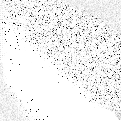
\includegraphics[width=\textwidth]{images/findings/round1/strategies_peggingmaxmedgained.png}
		\caption{\peggingmaxmedgained}
	\end{subfigure}
	~
	\begin{subfigure}[t]{0.22\textwidth}
		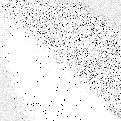
\includegraphics[width=\textwidth]{images/findings/round1/strategies_peggingminavggiven.png}
		\caption{\peggingminavggiven}
	\end{subfigure}

\caption{
	All final strategy strengths for Agent 0
	when playing as the dealer
	after training for one million games during Round 1.
}
% TODO: figure out axes
\label{fig_r1-strats}
\end{figure}


\subsubsection{Learning Results}

%%%
% Discuss Strategies Figure
%%%

%%%
Despite the all-or-nothing nature of how a single strategy is potentially
learned,
it is still worth noting that the agent did in fact learn to play different
strategies at different times.
%
As can be seen in Figure~\ref{fig:r1-strats},
the strengths of each strategy's weight do vary across score-locations.
%
For instance, when in the lead by
roughly two to twenty five points,
the agent will prefer to choose the hand with the most guaranteed
points in its own hand
by following \handmaxmin.
%
However, when the game is either extremely close
or when the agent is well in the lead,
the agent will take a slight gamble and play for expected points.
%
Occasionally, the agent will also attempt to pay attention to the points
gained through the play phase of a round by playing a combination that pegs
well.
%
Ironically,
the agent may play against its own best wishes by minimizing the average return
of the crib.
%
This is speculated to be a result of alignment of the results between
\cribminavg\ and more reasonable \handmaxmin\
or \handmaxavg.
%%%

%%%
Of further interest is how little the agent knows how to handle a losing
position.
%
As can be seen by looking in the upper-right half of each strategy's
individual graph,
of the explored losing states,
there is little consensus or pattern as to which strategy should dominate.
%
It is possible that agents which end up in these positions lose more often than
they win.
%
If this is the case,
the resulting punishment will decrease the top two or three strategies that were
most responsible for the hand choice at that state,
effectively increasing all others.
%
This in turn would likely later lead to a cycle in which different strategies
are cyclically placed in a role of strongest weight,
generating the fuzz seen now.
%%%


\subsubsection{Performance}

%%%
% TODO: discuss how it performed worse than random (got stonked)
While it is
aggravating that the agent learns to over-trust a single strategy,
it is simultaneously reassuring that general trends in play are detected.
%
However, the next metric
% TODO: test other agents against random
%%%


\subsubsection{Applications for Round 2}

%%%
% "Lessons Learned" / changes made
%	Learning rate lowered
%	exploration rate constant
%%%

%%%
% TODO: discuss how the meta-parameters were tweaked for round 2
%		and how the tournament structure got wonked
%%%

